\chapter{مبانی نظری توزیع کلید کوانتومی}
\label{chap:qkdtheory}
%=====================================================================

\section{اصول فیزیکی زیربنایی}

امنیت \lr{QKD} بر خلاف رمزنگاری کلاسیک، متکی به دشواری محاسباتی یک مسئلهٔ ریاضی نیست، بلکه مستقیماً از قوانین بنیادین مکانیک کوانتومی نتیجه می‌شود. دو اصل کلیدی در این میان نقش تعیین‌کننده دارند:

\begin{definition}[اصل عدم‌قطعیت در اندازه‌گیری]
اندازه‌گیری یک حالت کوانتومی ناشناخته در یک پایهٔ اندازه‌گیری دلخواه، به‌طور کلی آن حالت را برهم می‌زند؛ مگر آنکه پایهٔ اندازه‌گیری با پایه‌ای که حالت در آن تهیه شده، منطبق باشد.
\end{definition}

\begin{theorem}[قضیهٔ عدم-شبیه‌سازی \lr{\cite{wootters1982}}]
هیچ عملگر یکانی (فیزیکی) وجود ندارد که بتواند یک حالت کوانتومی دلخواه و ناشناخته $\lvert\psi\rangle$ را بدون تغییر در حالت اصلی، به‌طور کامل روی یک سامانهٔ کمکی کپی کند.
\end{theorem}

نتیجهٔ مستقیم این قضیه برای امنیت ارتباطات آن است که یک شنودگر \lr{(Eve)} \textbf{اصولاً نمی‌تواند} فوتون‌های حامل کلید را رهگیری، کپی و بدون تغییر ارسال کند؛ هرگونه تلاش برای اندازه‌گیری یا کپی‌برداری از حالت کوانتومی، اختلال آماری قابل‌کشفی در نرخ خطای بیت کوانتومی (تعریف در بخش \ref{sec:qberrate}) ایجاد می‌کند. این ویژگی، که در رمزنگاری کلاسیک هیچ مابه‌ازایی ندارد، پایهٔ \textbf{امنیت اثبات‌پذیر اطلاعاتی} \lr{(Information-Theoretic Security)} در \lr{QKD} است.

\section{پروتکل \lr{BB84}}

نخستین و پرکاربردترین پروتکل \lr{QKD}، پروتکل \lr{BB84}\LTRfootnote{Named after its inventors, Bennett and Brassard, and the publication year 1984.} است که در سال $1984$ توسط بنت و براسارد\LTRfootnote{Charles H. Bennett and Gilles Brassard} \lr{\cite{bennett1984}} پیشنهاد شد. شکل \ref{fig:bb84} گردش کار کلی این پروتکل را نشان می‌دهد.

\begin{figure}[htbp]
\centering
\begin{tikzpicture}[
  node distance=1.2cm,
  box/.style={rectangle,draw,thick,rounded corners,minimum width=2.6cm,minimum height=1cm,align=center,fill=blue!8},
]
\node[box] (alice) {\lr{Alice}\\\rl{(فرستنده)}};
\node[box,right=6.3cm of alice] (bob) {\lr{Bob}\\\rl{(گیرنده)}};
\draw[-{Stealth[length=3mm]},thick,blue!60!black] (alice) -- node[above,font=\footnotesize]{\rl{کانال کوانتومی (فوتون‌های تکی)}} (bob);
\draw[-{Stealth[length=3mm]},thick,red!60!black] ($(alice.south)+(0,-0.4)$) -- node[below,font=\footnotesize]{کانال کلاسیک (تطبیق پایه، تصحیح خطا، تقطیر محرمانگی)} ($(bob.south)+(0,-0.4)$);
\node[below=1.1cm of alice, align=right, font=\footnotesize] (a2) {\rl{\lr{1.} تولید بیت‌های تصادفی}\\\rl{\lr{2.} انتخاب تصادفی پایه ($+/\times$)}\\\rl{\lr{3.} کدگذاری و ارسال قوبیت‌ها}};
\node[below=1.1cm of bob, align=right, font=\footnotesize] (b2) {\rl{\lr{1.} انتخاب تصادفی پایهٔ اندازه‌گیری}\\\rl{\lr{2.} اندازه‌گیری قوبیت‌ها}\\\rl{\lr{3.} غربال‌سازی کلید \lr{(Key Sifting)}}};
\end{tikzpicture}
\caption{شمای کلی پروتکل \lr{BB84}: تبادل کلید کوانتومی بین \lr{Alice} و \lr{Bob}}
\label{fig:bb84}
\end{figure}

برای نمایش دقیق‌تر ترتیب زمانی پیام‌ها میان دو طرف، شکل \ref{fig:bb84seq} همان پروتکل را در قالب نمودار توالی \lr{(Sequence Diagram)} نشان می‌دهد که هفت گام اصلی توضیح داده‌شده در ادامه را به‌ترتیب دربر می‌گیرد.

\begin{figure}[htbp]
\centering
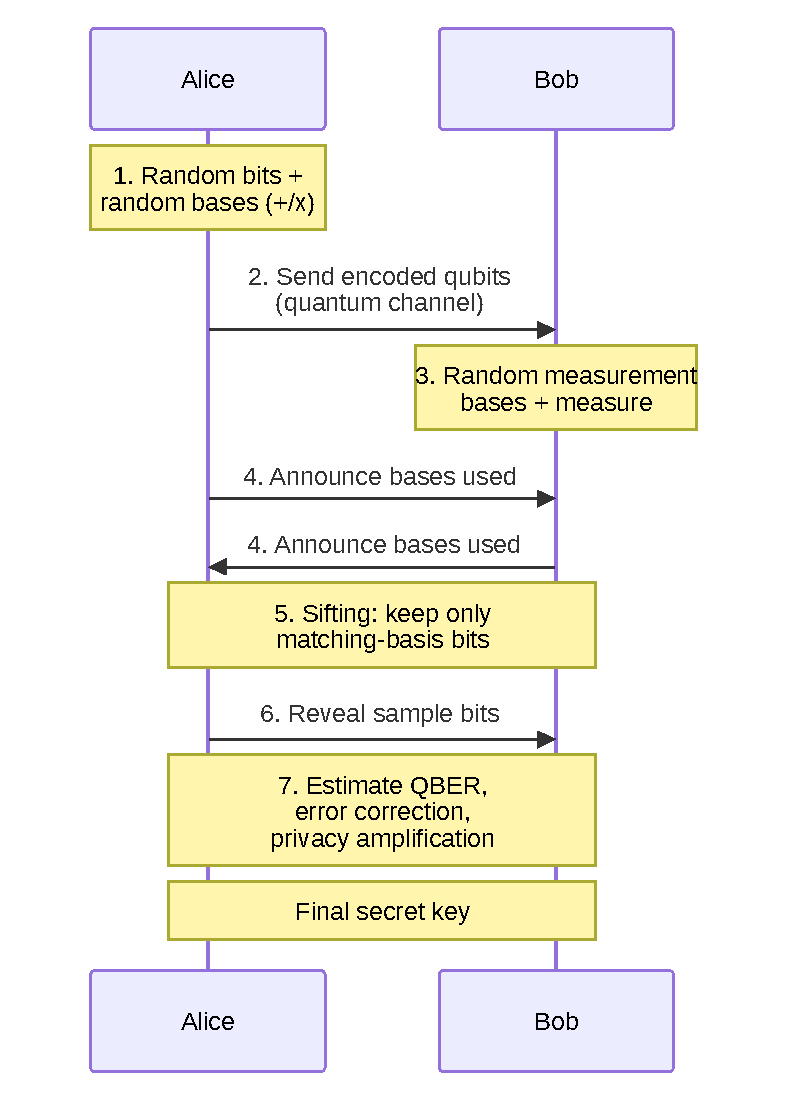
\includegraphics[width=0.75\linewidth]{figs/fig_bb84_sequence.pdf}
\caption{نمودار توالی زمانی پروتکل \lr{BB84} از تولید بیت تصادفی تا استخراج کلید نهایی}
\label{fig:bb84seq}
\end{figure}

مراحل اصلی پروتکل \lr{BB84} به شرح زیر است:

\begin{enumerate}
\item \textbf{تهیهٔ حالت \lr{(State Preparation)}:} \lr{Alice} برای هر بیت کلید، به‌صورت تصادفی یکی از دو پایهٔ متعامد، پایهٔ مستطیلی ($+$) یا پایهٔ قطری ($\times$)، را انتخاب کرده و بیت را روی حالت قطبش فوتون کدگذاری می‌کند.
\item \textbf{انتقال:} فوتون‌ها از طریق کانال کوانتومی (معمولاً فیبر نوری تاریک \lr{(Dark Fiber)} در طول‌موج $1550$ نانومتر یا کانال فضای آزاد/ماهواره‌ای) به \lr{Bob} ارسال می‌شوند.
\item \textbf{اندازه‌گیری:} \lr{Bob} برای هر فوتون دریافتی، به‌طور مستقل و تصادفی یکی از دو پایه را برای اندازه‌گیری انتخاب می‌کند.
\item \textbf{تطبیق پایه \lr{(Basis Reconciliation)}:} \lr{Alice} و \lr{Bob} از طریق یک کانال کلاسیک \textbf{احراز‌هویت‌شده} (نه لزوماً محرمانه)، پایه‌های انتخابی خود را، بدون افشای مقدار بیت‌ها، مقایسه کرده و تنها بیت‌هایی را نگه می‌دارند که در آن‌ها پایهٔ فرستنده و گیرنده یکسان بوده است. این مرحله «کلید غربال‌شده» \lr{(Sifted Key)} را تولید می‌کند.
\item \textbf{برآورد نرخ خطا و تصحیح خطا:} با مقایسهٔ زیرمجموعه‌ای تصادفی از کلید غربال‌شده، نرخ خطای بیت کوانتومی برآورد می‌شود.
\item \textbf{تقطیر محرمانگی \lr{(Privacy Amplification)}:} با استفاده از توابع درهم‌سازی جهانی \lr{(Universal Hashing)}، طول کلید کاهش داده می‌شود تا هرگونه اطلاعات نشت‌یافته به شنودگر عملاً به صفر برسد و «کلید نهایی امن» تولید شود.
\end{enumerate}

دو پایهٔ متعامد استفاده‌شده در گام تهیهٔ حالت، معمولاً به‌صورت قطبش خطی افقی/عمودی ($\lvert0\rangle$/$\lvert1\rangle$) برای پایهٔ مستطیلی، و قطبش مورب $45$/$135$ درجه ($\lvert+\rangle$/$\lvert-\rangle$) برای پایهٔ قطری، پیاده‌سازی می‌شوند؛ شکل \ref{fig:bb84states} این چهار حالت را در فضای قطبش نشان می‌دهد. ویژگی کلیدی این چهار حالت آن است که دو پایه نسبت به هم \textbf{مزدوج متقابل} \lr{(Mutually Unbiased Bases)} هستند: اندازه‌گیریِ یک حالت متعلق به یک پایه، با پایهٔ دیگر، نتیجه‌ای کاملاً تصادفی (با احتمال $50\%$) به همراه دارد. دقیقاً همین ویژگی است که تضمین می‌کند تلاش \lr{Eve} برای اندازه‌گیری بدون دانستن پایهٔ صحیح، اختلال آماری قابل‌کشفی در \lr{QBER} ایجاد کند.

\begin{figure}[htbp]
\centering
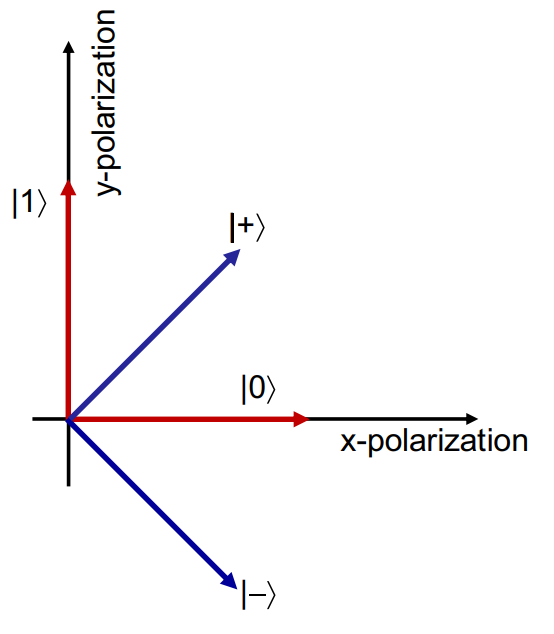
\includegraphics[width=0.5\linewidth]{figs/fig_bb84_states.png}
\caption{چهار حالت قطبش به‌کاررفته در پروتکل \lr{BB84}: دو حالت پایهٔ مستطیلی ($\lvert0\rangle,\lvert1\rangle$) و دو حالت پایهٔ قطری ($\lvert+\rangle,\lvert-\rangle$) \Cite{djordjevic2025pqc}.}
\label{fig:bb84states}
\end{figure}

\section{چالش منابع نوری واقعی: حملهٔ تقسیم تعداد فوتون و روش حالت فریب}
\label{sec:pns}

توضیح آرمانیِ پروتکل \lr{BB84} در بخش قبل، فرض را بر این می‌گذارد که \lr{Alice} برای هر بیت کلید، دقیقاً یک فوتون ارسال می‌کند. در عمل، ساخت یک منبع تک‌فوتونیِ واقعی \lr{(True Single-Photon Source)} که بتواند در نرخ بالا و با هزینهٔ معقول کار کند، همچنان چالشی مهندسی جدی است؛ به همین دلیل، اکثریت قریب‌به‌اتفاق سامانه‌های تجاری \lr{QKD} از یک لیزر متعارف که به‌شدت تضعیف شده است، یعنی \textbf{پالس همدوس ضعیف} \lr{(Weak Coherent Pulse, WCP)}، به‌عنوان جایگزین عملی استفاده می‌کنند. مشکل بنیادین این جایگزینی آن است که تعداد فوتون‌های گسیل‌شده در هر پالس از یک توزیع پواسون پیروی می‌کند، نه یک عدد ثابت؛ یعنی حتی وقتی میانگین تعداد فوتون در هر پالس ($\mu$) بسیار کوچک (برای نمونه $\mu \approx 0.1$) تنظیم شده باشد، همچنان احتمال غیرصفری وجود دارد که یک پالس معین حاوی دو یا چند فوتون باشد.

این احتمال کوچک اما غیرصفر، شکافی امنیتی خطرناک باز می‌کند که به \textbf{حملهٔ تقسیم تعداد فوتون} \lr{(Photon-Number-Splitting Attack, PNS)} معروف است \Cite{brassard2000limitations}. همان‌طور که شکل \ref{fig:pnsattack} نشان می‌دهد، \lr{Eve} می‌تواند یک تقسیم‌کنندهٔ پرتو \lr{(Beam Splitter)} در مسیر کانال کوانتومی قرار دهد: هر گاه پالسی حاوی بیش از یک فوتون از آن عبور کند، \lr{Eve} یکی از فوتون‌ها را جدا و در یک حافظهٔ کوانتومی ذخیره می‌کند، و بقیهٔ فوتون‌ها را بدون هیچ اختلالی به سمت \lr{Bob} عبور می‌دهد. \lr{Eve} حتی می‌تواند کانال را با فیبری با تلفات کمتر جایگزین کند تا افت شدت ناشی از این عملیات را جبران کند و کاملاً نامرئی بماند. پس از آنکه \lr{Alice} و \lr{Bob} پایهٔ صحیح را از طریق کانال کلاسیک اعلام کردند، \lr{Eve} همان پایه را روی فوتونِ ذخیره‌شدهٔ خود اعمال کرده و بیت را بدون ایجاد کوچک‌ترین خطای قابل‌کشفی در \lr{QBER} به‌دست می‌آورد؛ درست به همین دلیل است که فرمول نرخ کلید امن (رابطهٔ \eqref{eq:gllp}) صراحتاً میان رویدادهای \textbf{تک‌فوتونی} ($Q_1$، $e_1$) و نرخ کلی شمارش ($Q_\mu$، $E_\mu$) تمایز قائل می‌شود.

\begin{figure}[htbp]
\centering
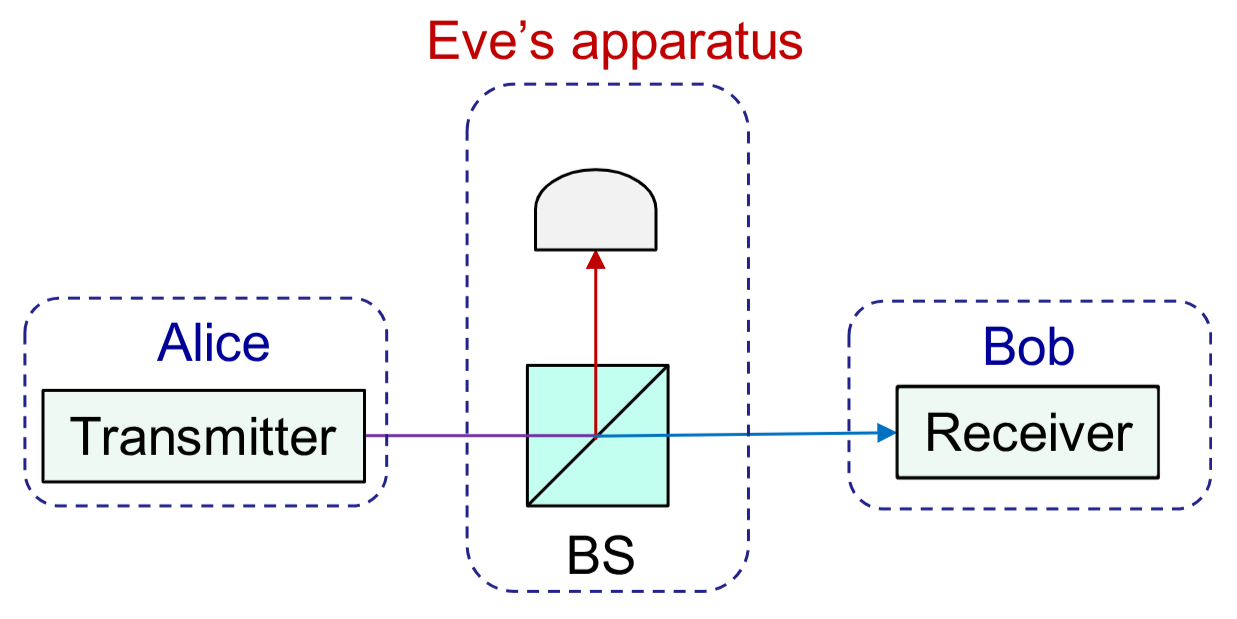
\includegraphics[width=0.7\linewidth]{figs/fig_pns_attack.png}
\caption{تصویرسازی حملهٔ تقسیم تعداد فوتون: \lr{Eve} با قراردادن یک تقسیم‌کنندهٔ پرتو \lr{(BS)} در مسیر، یکی از فوتون‌های اضافی پالس چندفوتونی را برداشت کرده و بقیه را بدون اختلال به \lr{Bob} می‌رساند \Cite{brassard2000limitations}.}
\label{fig:pnsattack}
\end{figure}

راه‌حل استاندارد صنعتی برای خنثی‌سازی این تهدید، \textbf{روش حالت فریب} \lr{(Decoy-State Method)} است \Cite{lo2005decoy}: به‌جای ارسال پالس‌هایی با شدت نوری ثابت، \lr{Alice} به‌طور تصادفی میان چند سطح شدت متفاوت (یک سطح «سیگنال» و یک یا چند سطح «فریب») جابه‌جا می‌شود، بدون آنکه از پیش مشخص کند کدام پالس متعلق به کدام سطح است. از آنجا که رفتار حملهٔ \lr{PNS} به‌شدت به تعداد فوتون موجود در هر پالس وابسته است، نرخ عبور \lr{(Transmittance)} مشاهده‌شده برای پالس‌های سیگنال و فریب، در غیاب شنود، باید از نظر آماری یکسان باشد. اگر \lr{Eve} حملهٔ \lr{PNS} را اجرا کند، از آنجا که او نمی‌تواند سطح شدت هر پالس را از پیش تشخیص دهد، رفتار متفاوتی نسبت به پالس‌های با شدت مختلف نشان می‌دهد و این تفاوت، پس از مقایسهٔ آماریِ نرخ عبور و نرخ خطای هر سطح شدت توسط \lr{Alice} و \lr{Bob}، حضور شنودگر را آشکار می‌سازد. این روش، بدون نیاز به منبع تک‌فوتونیِ واقعی، برد و نرخ کلید امن قابل‌دستیابی سامانه‌های \lr{WCP} را به‌طور چشمگیری افزایش داده است و امروزه در عملاً تمام سامانه‌های تجاری \lr{QKD} (شکل \ref{fig:qkdvendors}) به‌کار گرفته می‌شود.

\section{نرخ خطای بیت کوانتومی و نرخ کلید امن}
\label{sec:qberrate}

نرخ خطای بیت کوانتومی \lr{(Quantum Bit Error Rate, QBER)} مهم‌ترین شاخص کیفیت و امنیت یک پیوند \lr{QKD} است و به‌صورت زیر تعریف می‌شود:

\begin{equation}
\label{eq:qber}
\mathrm{QBER} = \frac{N_{\text{error}}}{N_{\text{total}}}
\end{equation}

که در آن $N_{\text{error}}$ تعداد بیت‌های نادرست در نمونهٔ آزمایش‌شده و $N_{\text{total}}$ تعداد کل بیت‌های غربال‌شدهٔ نمونه‌برداری‌شده است. در عمل، یک آستانهٔ امنیتی مشخص (برای \lr{BB84} معمولاً در حدود $11\%$) وجود دارد که فراتر از آن، امکان استخراج کلید امن از نظر تئوری اطلاعات وجود ندارد و ارتباط باید قطع شود.

با در نظر گرفتن اثرات عملی نظیر تلفات کانال، نویز آشکارساز و حملات نشت‌اطلاعات از کانال جانبی، نرخ کلید امن نهایی $R$ با فرمول تعمیم‌یافتهٔ \lr{GLLP}\LTRfootnote{Gottesman, Lo, Lütkenhaus, and Preskill} \lr{\cite{gllp2004}} به‌صورت زیر تخمین زده می‌شود:

\begin{align}
\label{eq:gllp}
R \;\geq\; q \Big\{ -Q_{\mu}\, f(E_{\mu})\, H_2(E_{\mu}) \;+\; Q_1 \big[1 - H_2(e_1)\big] \Big\}
\end{align}

که در آن $q$ کارایی پروتکل (برای \lr{BB84} با غربال‌سازی معمولی $q=1/2$)، $Q_{\mu}$ نرخ شمارش کلی، $E_{\mu}$ نرخ خطای کلی، $f(E_{\mu})$ کارایی الگوریتم تصحیح خطا (معمولاً بین $1.1$ تا $1.2$)، $Q_1$ و $e_1$ به‌ترتیب نرخ شمارش و نرخ خطای رویدادهای تک‌فوتونی، و $H_2(\cdot)$ تابع آنتروپی دودویی شانون است:

\begin{equation}
H_2(x) = -x\log_2(x) - (1-x)\log_2(1-x)
\end{equation}

این رابطه نشان می‌دهد که نرخ کلید امن با افزایش فاصلهٔ انتقال (و درنتیجه افزایش تلفات و کاهش $Q_1$) به‌صورت نمایی افت می‌کند، محدودیتی بنیادین که در فصل بعد، معماری‌های عملی برای غلبه بر آن معرفی می‌شوند.

%=====================================================================
